%==============================================================================%
%                               RAPPORT DE STAGE                               %
%==============================================================================%
% Auth: Rémi CHASSAGNOL                                                        %
% Desc: Rapport de stage de deuxième année à l'école l'ISIMA.                  %
%==============================================================================%

% Settings ---------------------------------------------------------------- {{{
\documentclass[a4paper]{article}

\usepackage[utf8]{inputenc}
\usepackage[T1]{fontenc}
\usepackage{textcomp}
\usepackage{url}
\usepackage{hyperref}
\usepackage[top=2.5cm,bottom=2.5cm,right=2cm,left=3cm]{geometry}
\usepackage[french]{babel}
\usepackage[backend=biber,style=ieee]{biblatex}
\usepackage{glossaries}
%\usepackage{titletoc}% http://ctan.org/pkg/titletoc
\usepackage{qtree}
\usepackage{listings}
\usepackage{xcolor}
\usepackage{setspace}
\usepackage{graphicx}
\usepackage{geometry}
\usepackage{titlesec}
\usepackage{chngcntr}
\counterwithin*{section}{part}

\addbibresource{refs.bib}

\definecolor{codegreen}{rgb}{0,0.6,0}
\definecolor{codegray}{rgb}{0.5,0.5,0.5}
\definecolor{backcolour}{rgb}{0.95,0.95,0.92}
\definecolor{backpink}{rgb}{1,0.94,0.95}

%===========style & geometry===========
%\lstset{style=mystyle}

 \geometry{
 a4paper,
  left=30mm,
  right=20mm,
  top=25mm,
  bottom=25mm,
 }

 \titleformat*{\section}{\LARGE\bfseries}
 \titleformat*{\subsection}{\Large\bfseries}

%================infos=================
\pagenumbering{gobble}
\begin{titlepage}

\title{Création d'un outil d'intégration continue}
\author{CHASSAGNOL Rémi}
\date{\today}
\end{titlepage}
%}}}
% Glossaire --------------------------------------------------------------- {{{
\makeglossaries
\newglossaryentry{ast}
{
    name=todo,
    description={le truc à faire}
}

%}}}

%------------------------------------------------------------------------------%
%                                   Document                                   %
%------------------------------------------------------------------------------%

\pagestyle{empty}
\begin{document}

% Title page -------------------------------------------------------------- {{{
\begin{titlepage}
  \hspace{\fill}
  \begin{figure}[!htb]
     \begin{minipage}{0.50\textwidth}
       \centering
       
\includegraphics[scale=0.8]{./img/logo_isima_inp.jpeg}
     \end{minipage}\hfill
     \begin{minipage}{0.50\textwidth}
       \centering
       
\includegraphics[scale=0.4]{./img/logo-ck.png}%
     \end{minipage}
  \end{figure}
  \begin{center}
    \vspace*{1cm}

    \par\noindent\rule{\textwidth}{0.5pt}
    \Huge
    \textbf{Création d'un outil d'intégration continue}
    \par\noindent\rule{\textwidth}{0.5pt}

    \vspace{0.2cm}
    \LARGE
    Rapport d'élève ingénieur\\
    Stage de $2^{ème}$ année\\
    Filière F2 : Génie Logiciel et Systèmes Informatiques

    \vspace{1.5cm}

    \large
    Présenté par : \textbf{Rémi CHASSAGNOL}

    \vfill

    \vspace{0.5cm}
  \end{center}


  \large
  \noindent
  Responsable ISIMA : Loïc YON \hfill \textbf{Soutenance: 30/08/2023}\\
  Responsable entreprise : Ludovic DESCOUT \hfill \textbf{Durée du stage: 5 mois}\\~\\
  \raggedright
  \begin{center}
  Campus des Cézeaux. 1 rue de la Chébarde. TSA 60125. 63178 Aubière CEDEX\\
  \end{center}
\end{titlepage}

\clearpage{}

%---------------------------------------------------------------------------}}}
% Table of Content -------------------------------------------------------- {{{
\pagenumbering{arabic}
\thispagestyle{empty}
\tableofcontents
\clearpage{}

%---------------------------------------------------------------------------}}}
% Remerciements ------------------------------------------------------------{{{
\section*{Remerciements}
\thispagestyle{empty}
\addcontentsline{toc}{section}{Remerciements}

\doublespacing

Les remerciements !!

\onehalfspacing

\clearpage{}

%---------------------------------------------------------------------------}}}
% Table des figures --------------------------------------------------------{{{
\listoffigures
\clearpage{}

%---------------------------------------------------------------------------}}}
% Résumé & Abstract --------------------------------------------------------{{{
%\setcounter{secnumdepth}{3}
\section*{Résumé}
\addcontentsline{toc}{section}{Résumé}

Le super résumer !
\\~\\

\noindent
Mots-clés : \textbf{C/C++}, \textbf{intégration continue}, \textbf{tests},
\textbf{systèmes embarqués}, \textbf{émulation}

\section*{Abstract}
\addcontentsline{toc}{section}{Abstract}

the amazing abstract
\\~\\

\noindent
Keywords : \textbf{C/C++}, \textbf{continuous integration}, \textbf{testing},
\textbf{embeded system}, \textbf{emulation}

\clearpage{}

%---------------------------------------------------------------------------}}}
% Introduction -------------------------------------------------------------{{{
\pagestyle{plain}
\setcounter{page}{1}
\clearpage
\section*{Introduction}
\addcontentsline{toc}{section}{Introduction}

Introduction

plan !

\clearpage{}

%---------------------------------------------------------------------------}}}

%------------------------------------------------------------------------------%
%                                     Plan                                     %
%------------------------------------------------------------------------------%

% Contexte du projet *******************************************************{{{
\part{Contexte du projet}

%% Présentation de CKsquare ================================================{{{
\section{Présentation de CKsquare}

CKsquare est une entreprise d'ingénierie spécialisée dans la conception de
systèmes de payement automatisés.

- monétique ++
- station auto lavage
- faite ses 20 ans cette année
- pousse les carte électroniques très loin -> solution très fiable / économique
  et écologique
- ils ont mis en place des systèmes perso pour pousser les cartes encore plus
  loin
- regroupement d'entreprises pour concevoir les bornes de A à Z
- fournissent des solution personnalisées pour les clients

%===========================================================================}}}
%% Tranvail demandé ========================================================{{{
\section{Travail demandé}

L'objectif du stage est de réaliser un outil permettant de pouvoir tester la
partie commune des bibliothèques qui s'exécutent sur les cartes électroniques
des bornes de la société. À terme, l'outil doit permettre de faire de
l'intégration continue, les tests doivent donc pouvoir être automatisés dans une
pipeline Gitlab.

La première tâche sera de trouver le framework de test adapté pour la conception
de l'outil. Le code à tester est écrit en C, cependant, la société souhaiterait
aussi pouvoir tester les bibliothèques écrites par l'équipe Qt. Il serait donc
intéressant que l'outil soit aussi adapté au C++.

Étant donné que les tests seront exécuter dans une pipeline (donc dans un
docker), il faudra s'assurer que le code puisse compiler sous Linux. De plus, le
code étant à la base fait pour s'exécuter sur une carte électronique, cela
nécessitera d'émuler les composants pour que le code puisse fonctionner
correctement. Il sera aussi nécessaire de simuler les interfaces permettant au
code d'interagir avec les composants émulés en utilisant différents protocoles
de communication comme le SPI ou encore le Cctalk. En plus de cela, il faudra
pouvoir remplacer une partie des bibliothèques de la carte pour pouvoir simuler
les composants.

Le résultat final doit être un outil qui doit pouvoir être facilement
réutilisable et adaptable. La documentation et la structure du code doit pouvoir
permettre d'aisément modifier ou copier les différents éléments. Par exemple, il
faudra que tous les composants simulés aient la même structure et que cette
structure soit suffisamment simple et générique pour pouvoir être copiée pour la
création d'un nouveau composant.

À noter que l'objectif du projet n'est pas d'écrire des tests. Des tests ont été
écrits durant le projet mais ces derniers ont pour objectif de valider le bon
fonctionnement des composants simulés et non celui du code de la société.

%===========================================================================}}}

\clearpage
%***************************************************************************}}}
% Réalisation et conception ************************************************{{{
\part{Réalisation et conception}

%% Choix du framework de test =============================================={{{
\section{Choix du framework de test}

Le but du projet est de concevoir un outil permettant de tester du code, la
première tâche à donc été de choisir un framework de test. Le framework de test
constitue la base de l'outil à créer, c'est donc un choix assez important. Dans
cette partie nous traiterons de la procédure qui a été utilisée pour trouver et
comparer des frameworks et des bibliothèques de test.

Étant donné le fait que le langage C est très utilisé, il y a beaucoup de choix
quand aux différentes bibliothèques de test utilisables. Le premier travail a
été de faire un listing des bibliothèques et frameworks de tests existants pour
ensuite pouvoir les comparer. Ce travail de recherche à permis de faire un prés
tri et d'éliminer les framework incomplets ou trop peut utilisés. Une fois le
listing terminé, il a fallut trouver des critères pour comparer les frameworks.

Tout d'abord, l'équipe de développement souhaitait pouvoir tester à la fois du
code \textbf{C} et du code \textbf{C++} pour pouvoir tester certaines parties de
code développées par l'équipe \textbf{Qt}. Ce critère était optionnel mais
apprécié. À noter que lorsque l'on parle de pouvoir tester du code C++, cela ne
prend pas seulement en compte le fait de pouvoir exécuter des fonctions basiques
puisque c'est parfaitement possible avec tous les frameworks C étant donné la
compatibilité entre le C et le C++. Pour pouvoir tester du code C++, il fallait
aussi que le framework soit capable d'interagir avec les structures de donnés
fournis par la bibliothèque standard de C++ ou encore de pouvoir traiter des
exceptions. Ce critère à aussi été considéré pour la recherche du framework et
des frameworks C++ on aussi été retenus..

Un autre critère concerne la modernité et la facilité d'utilisation du
framework. Cela peut sembler anodin mais l'écriture des tests est une tâche
aussi longue que le développement. Pour ne pas perdre de temps, il est
préférable que les tests soient le plus simple possible à mettre en place. De
plus, les tests peuvent aussi servir de documentation, c'est donc un avantage
non négligeable que d'avoir un framework qui permette d'écrire des tests
simples, lisibles et compréhensibles. Enfin, ce critère impacte aussi le temps
de conception de l'outil de test car le fait d'utiliser un framework trop
complexe aurait nécessité la conception de fonctions et macros (pour réduire la
complexité) et rallongé le temps d'écriture de la documentation.

TODO:
- statut du développement (star github, collaborateurs, dernière maj)

%===========================================================================}}}
%% Organisation du projet =================================================={{{
\section{Organisation du projet}

- myosismonnayeur
- fichiers de bases
  - Les fichiers locaux
  - Fichiers à tester (commun\_global, dev\_pic)
- les fichiers de Tests

%===========================================================================}}}
%% Simulation du stockage =================================================={{{
\section{Simulation du stockage}

%%% Interface I²C ----------------------------------------------------------{{{
\subsection{Interface I²C}


%---------------------------------------------------------------------------}}}
%%% Interface SPI ----------------------------------------------------------{{{
\subsection{Interface SPI}


%---------------------------------------------------------------------------}}}

%===========================================================================}}}
%% Simulation des composants ==============================================={{{
\section{Simulation des composants}

%%% Interface Cctalk -------------------------------------------------------{{{
\subsection{Interface Cctalk}


%---------------------------------------------------------------------------}}}
%%% Interface MDB ----------------------------------------------------------{{{
\subsection{Interface MDB}


%---------------------------------------------------------------------------}}}

%===========================================================================}}}
%% Déroulement du projet ==================================================={{{
\section{Déroulement du projet}

%%% Les outils -------------------------------------------------------------{{{
\subsection{Les outils utilisés}

%%%% Gestion de version ....................................................{{{
\subsubsection{Gestion de version}

utilisation de git / version modifiée de gitflow. Je suis seul mais j'ai quand
même organiser mes branche de façon similaire à gitflow pour ne jamais casser du
code qui marche en mergant ou en tentant d implémenté du code qui marche pas.

%...........................................................................}}}
%%%% Gitlab ................................................................{{{
\subsubsection{Gitlab}

ci/cd

%...........................................................................}}}
%%%% Compilation ...........................................................{{{
\subsubsection{Compilation}

L'objectif étant de pouvoir automatiser les tests dans une pipeline Gitlab, il
fallait obligatoirement que les tests puissent compiler sur un docker et donc
sur un Linux. L'outil le plus adapté pour ce genre de tache est
\textbf{Makefile} qui a été utilisé en début de projet. Le défaut de Makefile
est qu'il reste assez proche du script et qu'il faut obligatoirement détailler
toutes les commandes. Étant donné le fait qu'il y avait beaucoup de fichiers, le
Makefile est vite devenu très compliqué et illisible et ce même si aucune
compilation séparé n'a été mise en place au début du projet. Quand de plus en
plus de fichiers ont été ajoutés au projet de test, il a fallut mettre en place
de la compilation séparée pour ne pas tout recompiler à chaque fois. Faire cela
avec Makefile est tout à fait possible mais cela aurait pris beaucoup de temps     % rep cela
et le fichier final aurait été assez peu lisible et surtout assez compliqué à
comprendre. Le but étant de faire un outil facilement compréhensible et
utilisable par tous les membres de l'entreprise, il fallait trouver une solution
plus simple. La syntaxe de \textbf{CMake} à permis de simplement lister les
fichiers à compiler ainsi que les répertoires à inclure sans avoir besoin de
détailler les option de gcc. Cet outil permet de générer un Makefile complet
avec un syntaxe beaucoup plus simple. De plus, CMake permet nativement de faire
de la compilation séparer ce qui à permis de gagner du temps pendant le
développement étant donner le fait que seuls les fichiers modifiés sont
recompilés lors de l'écriture des tests.

%...........................................................................}}}
%%%% nvim ..................................................................{{{
\subsubsection{nvim}

I use vim btw

%...........................................................................}}}

%---------------------------------------------------------------------------}}}
%%% Planification des tâches -----------------------------------------------{{{
\subsection{Planification des tâches}

On voit ça sur le gantt.

Ce diagramme est disponible en index \ref{appendix:expectedgantt} pour
plus de lisibilité.

% [expected gantt] {{{
% \begin{figure}[h!]
%   \begin{center}
%   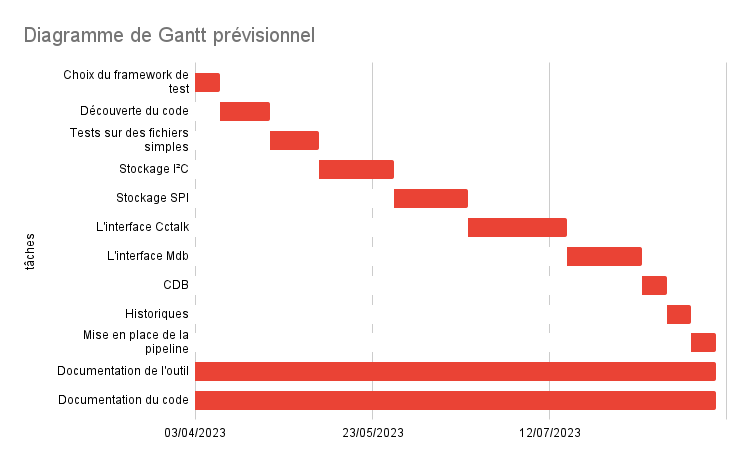
\includegraphics[scale=0.35]{./img/expected-gantt.png}
%   \caption{Diagramme de Gantt prévisionnel}
%   \end{center}
% \end{figure}
%}}}

Mais en fait on a fait ça parceque

On peut retrouver ce diagramme en index \ref{appendix:realgantt}.

% [real gantt] {{{
% \begin{figure}[h!]
%   \begin{center}
%   \includegraphics[scale=0.35]{./img/real-project.png}
%   \caption{Diagramme de Gantt réel.}
%   \end{center}
% \end{figure}~\\
%}}}

conclusion

%---------------------------------------------------------------------------}}}
%===========================================================================}}}

\clearpage
%***************************************************************************}}}
% Résultats et discussions *************************************************{{{
\part{Résultats et discussions}

%% TODO ===================================================================={{{
\section{TODO}

todo

\clearpage
%===========================================================================}}}
%% Discussion et perspectives =============================================={{{
\section{Discussion et perspectives}

On a fait ça et c'est bien mais on pourrait faire ça ou changer ça.

\clearpage
%===========================================================================}}}
%% Conclusion =============================================================={{{
\section*{Conclusion}
\addcontentsline{toc}{section}{Conclusion}

CONCLUSION

%}}}

%***************************************************************************}}}

%------------------------------------------------------------------------------%
%                                 bibliography                                 %
%------------------------------------------------------------------------------%

\begin{itemize}
  \item \cite{mankar2014review}: présentation du protocole I²C
  \item \cite{dhaker2018introduction} et \cite{li2014design}: présentation du
    protocole SPI
  \item \cite{engblom2015continuous}: simulation pour CI sur systèmes embarqués
  \item \cite{maartensson2016continuous}: intégration continue sur les systèmes
    embarqués.
\end{itemize}

\clearpage{}
\pagestyle{empty}
\printbibliography[keyword={paper},title={Biliographie}]
\printbibliography[keyword={web},title={Webographie}]

%------------------------------------------------------------------------------%
%                                  glossaire                                   %
%------------------------------------------------------------------------------%
\clearpage
\printglossaries

%------------------------------------------------------------------------------%
%                                   annexes                                    %
%------------------------------------------------------------------------------%
\appendix

% Diagramme de Gantt prévisionnel ------------------------------------------{{{
\clearpage{}
\section{Diagramme de Gantt prévisionnel}\label{appendix:expectedgantt}

% \begin{figure}[h!]
%   \begin{center}
%   \rotatebox[origin=c]{90}{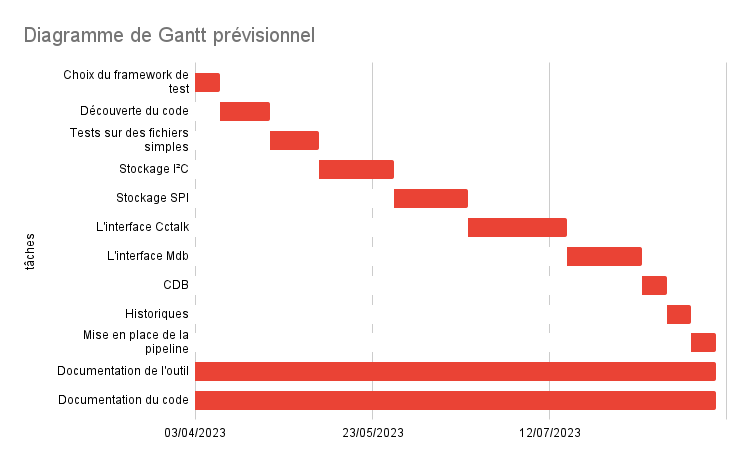
\includegraphics[scale=0.5]{./img/expected-gantt.png}}
%   \caption{Diagramme de Gantt prévisionnel.}
%   \end{center}
% \end{figure}
%---------------------------------------------------------------------------}}}
% Diagramme de Gantt réel --------------------------------------------------{{{
\clearpage{}
\section{Diagramme de Gantt réel}\label{appendix:realgantt}

% \begin{figure}[h!]
%   \begin{center}
%   \rotatebox[origin=c]{90}{\includegraphics[scale=0.5]{./img/real-project.png}}
%   \caption{Diagramme de Gantt réel.}
%   \end{center}
% \end{figure}
%---------------------------------------------------------------------------}}}

\end{document}
